\documentclass[manuscript,screen,review, 12pt, nonacm]{acmart}
\let\Bbbk\relax % Fix for amssymb clash 
\usepackage{vmlmacros}
\AtBeginDocument{%
  \providecommand\BibTeX{{%
    \normalfont B\kern-0.5em{\scshape i\kern-0.25em b}\kern-0.8em\TeX}}}
\usepackage{outlines}
\setlength{\headheight}{14.0pt}
\setlength{\footskip}{13.3pt}
\title{An Alternative to Pattern Matching, Inspired by Verse}

\author{Roger Burtonpatel}
\email{roger.burtonpatel@tufts.edu}
\affiliation{%
\institution{Tufts University}
\streetaddress{419 Boston Ave}
  \city{Medford}
  \state{Massachusetts}
  \country{USA}
  \postcode{02155}
  }
\begin{document}
  

\section{\VMinus can be compiled to a decision tree}
\label{vminustod}
    To demonstrate that \VMinus has the same desirable cost model as pattern
    matching, I present an algorithm for compiling \VMinus to a decision tree. I
    choose the decision tree as a target for compilation for the simple reason
    of its appealing cost model. A decision tree can be exponential in size but
    never examines a word of the \it{scrutinee}--- the value being tested---
    more than once. It is the compilation from \VMinus to \D that establishes
    this property by ensuring that no \it{test} node \it{T} has any proper
    ancestor \it{T'} such that \it{T} and \it{T'} both test the same location in
    memory.   

    This compilation algorithm serves to demonstrate that \VMinus is a viable
    alternative to pattern matching on the grounds that they have equivalent
    cost models: pattern matching can be compiled to a decision tree,
    which~\citet{macqueen1985tree} built the foundation for and~\citet{maranget}
    expanded on. 

    The algorithm runs during \DTran, the transformation from \VMinus to \D. Its
    domain, instead of a \it{case} expression, is \VMinus's \it{if-fi}. 
       
    \subsection{\D is a generalization of Maranget's trees} 

  \D's concrete syntax is given in Figure~\ref{fig:dsyntax}. Decision trees in \D
    are engineered to look like Maranget's trees. There are a few minor
    differences in the algorithm I use and Maranget's: his compilation algorithm
    is more complex than the one in this paper, and involves an intermediate
    representation of occurrence vectors and clause matrices which the algorithm
    I present does not use. Maragnet uses vectors and matrices to express
    multiple simultaneous matches of values to patterns as a single match of a
    vector with a matrix row. This allows him to run a \it{specialization} pass
    that reduces the number of rows in the matrix, ultimately leading to smaller
    trees.
    
        
    The underlying structures of Maranget's and \D's decision trees, however,
    are analogous. The same operation is the heart of their evaluation: they
    take a value, examine it, and choose a branch based on its form (Maranget
    calls the operation \textsc{Switch}; we call it \it{test}). 

    Let's look at an example from \it{Compiling Pattern Matching to Good
    Decision Trees} which shows the structure of a simple pattern-matching
    function and its corresponding decision tree.
    % , then at a corresponding tree
    % in \D. 

    Maranget beings with the function, \tt{merge}, which merges two lists: 

    \begin{figure}[H]
        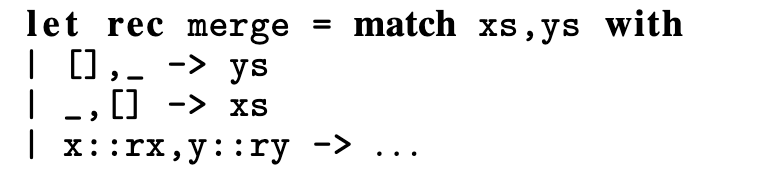
\includegraphics[scale=0.7]{../images/merge.png}
        \Description{Maranget's merge implementation}
        \caption{The skeleton of Maranget's \tt{merge}}
    \end{figure}

    % He then shows an intermediate representation in his compilation algorithm,
    % the occurrence vector and clause matrix: 

    % \begin{figure}[H]
    %     \begin{gather*}
    %         \vec{o} = (\tt{xs ys}) \hspace{3em}
    %         P \rightarrow A = 
    %         \begin{pmatrix}
    %             \tt{[]}     & \tt{\_}     & \rightarrow \tt{xs} \\
    %             \tt{\_}     & \tt{[]}     & \rightarrow \tt{ys} \\
    %             \tt{\_::\_} & \tt{\_::\_} & \rightarrow \tt{...} 
    %         \end{pmatrix}
    %     \end{gather*}


    %     \Description{Occurrence vector of names, and clause matrix of matches}
    %     \caption{The occurrence vector and clause matrix are intermediate
    %     representations in Maranget's compilation. I do not exploit this
    %     representation in my own algorithm, but it helps to understand his final
    %     tree.}
    % \end{figure}

    He compiles the function to this decision tree: 

    \begin{figure}[H]
        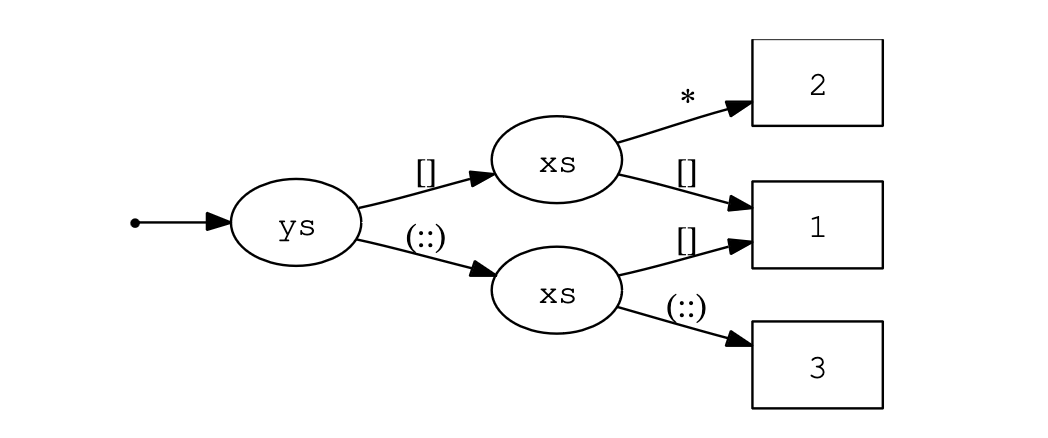
\includegraphics[scale=0.7]{../images/dtree.png}
        \Description{The final decision tree for merge} 
        \caption{The final compiled decision tree for \tt{merge}, right-to-left}
    \end{figure}

    When presented with the values \tt{xs} and \tt{ys}, the tree first tests
    \tt{xs} against its two known possible forms: the nullary list constructor
    \tt{[]}, and the application of the \it{cons} constructor \tt{::}. If
    \tt{xs} is equal to \tt{[]}, the tree immediately returns \tt{ys}. If
    \tt{xs} is an application of \tt{::}, the tree then tests \tt{ys} against
    the same list of possible constructors, and returns a value according to the
    result of the match. Each time the tree goes down a \tt{::} branch, it can
    extract the arguments of the \tt{::} for later use: these are \tt{x},
    \tt{y}, \tt{xr}, and \tt{yr}, which are used in the \tt{...} branch. This
    process of extracting arguments generalizes to all value constructors with
    one or more arguments. 

    \begin{figure}
      \begin{center}
      \dcsyntax
      \end{center}
      \Description{The concrete syntax of D.}
      \caption{\D: Concrete syntax}
      \label{fig:dsyntax}
      \end{figure}

    % Here is the decision tree for \tt{merge} in \D. 

    % \begin{figure}[H]
    %   \centering
    %     \it{Like the semantics, this figure is in progress.}
    %     \Description{The decision tree for merge, now in D} 
    %     \caption{The tree for \tt{merge} in D looks similar to Maragnet's.}
    % \end{figure}

    In \D, an \it{extract} node extract all from a value constructor at once for
    use in subtrees. The compiler is responsible for introducing the fresh names
    used in \it{extract}. 

    In \D, like in \VMinus, expressions can \it{fail}, meaning some of \D's 
    syntactic forms like \it{try-let} and \it{cmp} need an additional 


    \subsection{Rules (Big-step Operational Semantics) for \D:}
    \label{desemantics}
    
    \rab{The semantics for \D are being revised.}
    % \dsemantics
    \subsection{The \DTran\ algorithm: \VMinus $\rightarrow$ \D}

    \algrenewcommand\algorithmicwhile{\bf{let }}
    \algrenewcommand\algorithmicdo{\bf{in }}
    \algrenewcommand\algorithmicend{\bf{end}}
    \newcommand\alet\algorithmicwhile
    \newcommand\ain\algorithmicdo
    \newcommand\aend\algorithmicend

    \newcommand\branches{\ensuremath{\mathit{branches}}}
    \newcommand\compile{\ensuremath{\mathit{compile}}}
    \newcommand\mg{\ensuremath{-}}


    When presented with an \it{if-fi}, \DTran\ calls the function \compile,
    whole algorithm is presented in Figure~\ref{dtran}. \DTran\ first introduces
    all the names under the all existential $\exists$'s to a context which
    determines if a name is \it{known} or \it{unknown}. At the start, each name
    introduced by $\exists$ is \it{unknown}. Since all names are unique at this
    stage, there are no clashes. \DTran\ also desugars choice to multiple
    \it{if-fi} branches with a desugaring function \ITran: 

    \itran{if\; \dots \square\; gs_{1};\; \choiceg{gs_{2}}{gs_{3}};\; gs_{4} \rightarrow e\; \square \dots \;fi}
    
    ==
    
    ${if\; \dots \square\; gs_{1};\; gs_{2} \rightarrow e \;\square\; gs_{3};\; gs_{4} \rightarrow e \;\square \dots \;fi}$


    With the new context and desugared \it{if-fi}, \compile\ then repeatedly
    chooses a guarded expression $G$ and attempts the following while
    translating $G$'s internal expressions with \DTran: 

    \begin{enumerate}
        \item If there are no guards in $G$, insert a \it{match} node with the
        right-hand side of $G$. 
        \item Otherwise, choose an equation in $G$ of the form $x = K \dots$
        s.t. $x$ is \it{known}. 
        \item If one is found, use it to generate a \it{test} node, building
        each subtree of the \it{test} by pruning all branches in \it{all}
        guarded expressions of the \it{if-fi} in which $x = e$ and $e \neq K
        \dots$ and invoking \compile\ on the remaining ones with a context where
        $x$ is known. Each of these remainders is the child of an \it{extract}
        node which extracts the internals of each possible value constructor
        into a list of names which are introduced to the context. The algorithm
        builds the default tree of the \it{test} by finding any branches of the
        in the \it{if-fi} in which $x$ is not bound to a value constructor. 
        \item If no equation of the form \it{x = K \dots} is found, try to find
        an equation $x = e$ s.t. either $x$ is unknown and all names in $e$ are
        known. 
        \item If one is found, use it to generate a \it{try-let} node with two
        children: one if binding succeeds, and one if $e$ fails. \compile prunes
        each subtree of the \it{try-let} accordingly.
        \item If no equation is found, try to find an equation $x = y$ s.t. $x$
        is known and $y$ is unknown. 
        \item If one is found, use it to generate a \it{try-let} node with one
        child for when binding succeeds. \compile prunes the subtree of all 
        instance of $x = y$. 
        \item If no such equation is found, try to find a condition $e$ s.t. all
        names in $e$ are known. 
        \item If one is found, generate a fresh name $x'$ and use it to generate
        a \it{try-let} node for the equation $x = e'$, pruning each subtree of
        $e$ with a substitution of $[x/e]$. 
        \item If no condition $e$ is found, try to find an equation $x = e$ s.t.
        both $x$ and all names in $e$ are \it{known}.
        \item If one is found, generate a \it{cmp} node, prune the \it{if-fi} of
        all duplicate instances of that $x = e$, and invoke \compile again. 
        \item If none is found, the \it{if-fi} cannot be compiled to a decision
        tree. The algorithm halts with an error. 
    \end{enumerate}
    \raggedbottom

    The algorithm terminates when inserts a final \it{match} node for a
    right-hand side expression $e$ when the list of guards preceding $e$ is
    empty or a list of assignments from names to unbound names. Termination of
    \DTran\ is guaranteed because each recursive call passes a list of guarded
    expressions in which the number of guards is strictly smaller, so eventually
    the algorithm reaches a state in which the first unmatched branch is all
    trivially-satisfied guards. 

    In the figure, I use the notation $x@b$ to denote the bag of all guards and
    expressions in branch $b$ in which name $x$ appears. A branch is a list of
    guards followed by a terminal expression; it is a branch of an \it{if-fi}
    stripped of the existential since \DTran\ introduces all names at the top
    level. I use the notation $\dom(b)$ to describe the set of all names that
    appear in a branch. I use the notation $\mathit{branches -- g}$ to mean
    “$\mathit{branches}$ pruned of guard $g$” and the notation $\mathit{branches
    --- g}$ to mean “$\mathit{branches}$ pruned of all \it{branches} containing
    $g$.” I use the standard substitution notation $\mathit{branches[x/e]}$ to
    mean “$\mathit{branches}$ with name $x$ substituted for expression $e$.” I
    use a shorthand $\mathit{(context + \bracketed{n_1 \dots n_i \mapsto
    known})}$ to mean “$\mathit{context}$ extended with each of $n_x$ bound to
    $\mathit{known}$. 

    Not show in the algorithm is the case where \compile\ cannot choose a $g$ of
    one of the valid forms; in this case, \compile\ halts with an error. This
    can happen when no $g$ is currently solvable in the context, as determined
    by the same algorithm that \VMinus uses to pick a guard to solve, or when
    the program would be forced to unify incompatible values, such as any value
    with a lambda. 

    % \DTran\ makes the distinction for an equation \it{x = e}
    % based off of this model: 
    % \begin{enumerate}
    % \item 
    % \end{enumerate}
    % No guards  ==  MATCH
    % CONDITION  ==   if known, convert to LET, IF
    % EQN (x, e) ==
    %    - if x is known and e is VCONAPP, generate TEST
    %    - if x is known and e is not VCONAPP and e is known
    %         generate LET, IF
    %    - if x is unknown and e is known, then generate LET
       
%  What if we don't find any of the above? 
%  There must be only unknown guards. 
%  Can't compile! 
    
    % For an equation that
    % represents a binding of values to values, the algorithm inserts a \it{let}
    % node, and for a condition guard \it{e}, it inserts a \it{let} followed by 
    % an \it{if-then-else}. 
    
  
    \begin{figure}[H]
      \scriptsize
        \begin{algorithmic}
\Require $\forall (n : \rm{name})\; \in \branches, \; n\; \rm{unique}$
\State \it{compile context \branches} = 
  \If{\it{null(\branches)}} {\it{fail}}
  \ElsIf{$\neg\exists{g} \in$ \it{fst(hd(\branches))}} 
    \State {\it{match (hd branches)}}
  \Else
    \State \alet $g$ be a guard such that $g \in \branches$
    \ain 
    \If{$g$ has the form $x = K (e_1 \dots e_i)$}
    \alet 
    \State 
    $\mathit{KS = \bracketed{K\; \vert\; \exists\; b \in \branches : x \in \dom(b) \wedge K(\dots) \in x@b }}$ 
        
    $\mathit{edges = map(}$ 
    \State $\mathit{\lambda K.}$ (\alet $ns = n_1 \dots n_i, \; n_x \rm{ fresh}$
        \ain 
        \State $\mathit{(K, extract (x, ns, \compile (context + \bracketed{n_1 \dots n_i \mapsto known})}$ 
        \State $\mathit{(mapPartial (refine\; x\; (K (ns))) branches))}$ 
        \State \aend) 
      \State $\mathit{defaults = filter(\lambda b. x \notin \dom(b) \lor K(\dots) \notin x@b)}$ 
      \State \ain $\mathit{test (x, edges, SOME (compile\; defaults))}$ 
      \State \aend 
    \ElsIf {$g$ has the form $x = e$ : $x \;\mathit{unknown},\; e \;\mathit{known}$} 
      \State $\mathit{try\_let (x, \DTran\; (context\; e)}$, 
      \State $\mathit{compile (context\bracketed{x \mapsto known}) ((branches -- eq)[x/e])}$,
      \State $\mathit{SOME (compile\; context\; (branches --- eq --- e)))}$
    \ElsIf {$g$ has the form $x = y$ : $x \;\mathit{known},\; y \;\mathit{unknown}$} 
    \State $\mathit{try\_let (x, y, compile (context\bracketed{y \mapsto known}) (branches -- eq), NONE)}$
    \ElsIf {$g$ has the form $x = e$ : $x \;\mathit{known},\; e \;\mathit{known}$} 
      \State $\mathit{cmp (x, \DTran\; (context\; e)}$, 
      \State $\mathit{compile\; context\; ((branches -- eq)[x/e])}$,
      \State $\mathit{compile\; context\; (branches --- eq -- e)}$,
      \State $\mathit{SOME (compile\; context\; (branches --- eq --- e)))}$
    \ElsIf {$g$ has the form $e$ : $e \;\mathit{known}$} 
    \State $\mathit{try\_let (x, \DTran\; (context\; e)}$, 
    \State $\mathit{compile (context\bracketed{x \mapsto known}) ((branches -- eq)[x/e])}$,
    \State $\mathit{SOME (compile\; context\; (branches --- eq --- e)))}$ 
    \State {, $x$ fresh} \\
    \aend
    \EndIf
  \EndIf
  \State \bf{where} 
  \State $\mathit{snd (a, b) = b}$ 
  \State $\mathit{refine (x, K (ns) b) = }$
  \If{$\mathit{K' (es) \in x@b \land (K \neq K' \lor length(es) \neq length(ns))}$}
        $\mathit{NONE}$
  \Else $\;\mathit{SOME\; b}$
  \EndIf 

\end{algorithmic}
    \Description{The \DTran\ algorithm} 
    \caption{The \DTran\ algorithm.}
    \label{dtran}
    \end{figure}    



    \subsection{Translation from \VMinus to \D preserves semantics}
    
    Translating \it{if-fi} to a decision tree should preserve semantics. The
    following theorem formalizes this claim: 

    \begin{proof}
        See appendix A. 
    \end{proof}

\end{document}